\subsection{Datum}
\subsubsection{Gedrag}
Na een reset of \'e\'en keer per dag om 12 uur middernacht zal het datum component de data voor de nieuwe datum verzenden naar de zend buffer. De inkomende data is in het binary coded decimal (bcd) formaat. Eerst zal hij de dag van de week doorgeven, daarna de dag van de maand, de maand en daaropvolgend het jaartal. Dat allemaal sequentieel, getriggert op de neergaande klokflank van de ready_buf. 

\begin{figure}
  \centering
     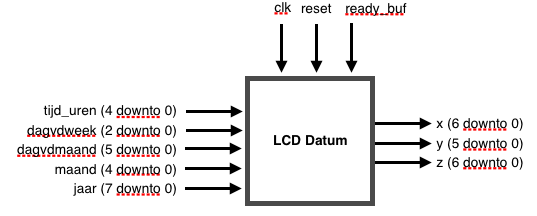
\includegraphics[angle = 0, scale= 0.75]{verslag_schemas/datum_entity.png}
       \caption{Entity datum}
\label{fig:simlayout}
\end{figure}


\subsubsection{Functionaliteit}
Het component werkt met een finite state machine (FSM) en een apart process om de juiste input te bepalen. \\
Na de reset zal het process in 

\subsubsection{FSM}
\begin{figure}
  \centering
     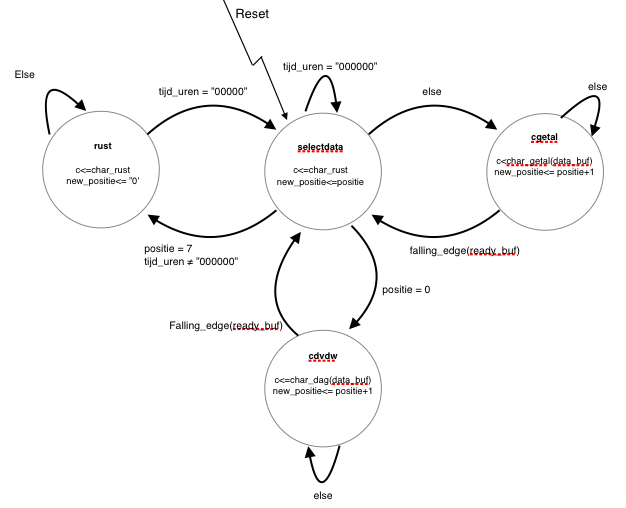
\includegraphics[angle = 0, scale= 0.75]{verslag_schemas/datum_fsm.png}
       \caption{FSM Datum}
\label{fig:simlayout}
\end{figure}

\subsubsection{VHDL code}

\subsubsection{Simulaties}

\subsubsection{Testen}

\subsubsection{Resultaten}

\subsubsection{Discussie}
